Dans ce chapitre, nous enrichissons le langage défini dans le
chapitre~\ref{cha:lang} d'un système de types. Celui-ci permet de séparer les
programmes bien formés, comme celui de la figure~\ref{fig:progwf:good} des
programmes mal formés comme celui de la figure~\ref{fig:progwf:bad}.

\begin{SaveVerbatim}[]{VerbProgGood}
f = Fun() {
  Decl x = 0 in
  x <- 1
  return x
}
\end{SaveVerbatim}

\begin{SaveVerbatim}[]{VerbProgBad}
f = Fun() {
  Decl x = 0 in
  x <- 1
  return (*x)
}
\end{SaveVerbatim}

\begin{figure}[h]

  \centering

  \subbottom[Programme bien formé]{
\label{fig:progwf:good}
    \begin{minipage}{5cm}
    \BUseVerbatim{VerbProgGood}
    \end{minipage}
  }
  \hspace{2cm}
  \subbottom[Programme mal formé]{
\label{fig:progwf:bad}
    \begin{minipage}{5cm}
    \BUseVerbatim{VerbProgBad}
    \end{minipage}
  }

  \caption{Programmes bien et mal formés}
\label{fig:progwf}

\end{figure}

Le but d'un tel système de types est de rejeter les programmes pour lesquels ont
peut facilement déterminer qu'ils sont faux, c'est-à-dire dont on peut prouver
qu'il provoqueraient des erreurs à l'exécution dues à une incompatibilité entre
valeurs. En ajoutant cette étape, on restreint la classe d'erreurs qui
pourraient bloquer la sémantique.

On emploie un système de types monomorphe: à chaque expression, on associe un
type, et non un schéma de types. Il y a deux exceptions : tout d'abord, le
pointeur $\eNull$ a pour type $t~*$. Mais cela ne pose pas de complications, car
il n'y a pas d'étape de généralisation de $t$. Cela indique seulement que
$\eNull$ est compatible avec n'importe quel type pointeur. L'autre cas concerne
les tests d'égalité, qu'on veut pouvoir faire sur les valeurs de types scalaires
et tous les types qui sont composés de ces types (on veut par exemple éviter de
tester l'égalité de deux fonctions). Là encore, cela ne pose pas de problème,
puisqu'on peut statiquement savoir si un type a cette propriété ou pas.

En plus des types de base $\tInt$, $\tFloat$ et $\tUnit$, on peut construire des
types composés: pointeurs, tableaux, structures et fonctions.

Pour typer les structures, on suppose avoir à notre disposition (par un
prétraitement, par exemple) le type complet de la structure à chaque accès d'un
champ. Cela alourdit la présentation, mais permet d'éviter le sous-typage qui
rend l'inférence indécidable. En pratique, dans l'implantation décrite dans le
chapitre~\ref{cha:implem}, on utilise une variante du polymorphisme de rangée
(\emph{row polymorphism}) présent dans OCaml pour unifier deux types structures
partiellement connus.

Le principe du typage est d'associer à chaque construction syntaxique une
étiquette représentant le genre de valeurs qu'elle produira. Dans le programme
de la figure~\ref{fig:progwf:good}, la variable $x$ est initialisée avec la
valeur $0$, c'est donc un entier. Cela signifie que dans tout le programme,
toutes les instances de cette variable
\footnote{Deux variables peuvent avoir le même nom dans deux fonctions
  différentes, par exemple. Dans ce cas il n'y a aucune contrainte particulière
  entre ces deux variables. L'analyse de typage se fait toujours dans un
  contexte précis.
}
porteront ce type. La première instruction est l'affectation de la constante $1$
(entière) à $x$ dont on sait qu'elle porte des valeurs entières, ce qui est donc
correct. Le fait de rencontrer $\iReturn{x}$ permet de conclure que le type de
la fonction est $(~) → \tInt$.

Dans la seconde fonction, au contraire, l'opérateur $*$ est appliqué à $x$ (le
début de l'analyse est identique et permet de conclure que $x$ porte des valeurs
entières). Or cet opérateur prend un argument d'un type pointeur de la forme
$t*$ et renvoie alors une valeur de type $t$. Ceci est valable pour tout $t$
($\tInt$, $\tFloat$ ou même $t'*$: le déréférencement d'un pointeur sur pointeur
donne un pointeur), mais le type de $x$, $\tInt$, n'est pas de cette forme. Ce
programme est donc mal typé.

Dans ce chapitre, on commence par poser les notations qui vont servir à définir
la relation de typage. Ensuite, on explique les différentes règles de typage sur
les composantes de \langname: expressions, instructions et phrases. Enfin, dans
le reste du chapitre on établit des propriétés qui sont respectées par les
programmes bien typées. On conclut par les théorèmes de progrès et de
préservation qui établissent la sûreté du typage.

\section{Environnements et notations}

Les types associés aux expressions sont décrits dans la
figure~\ref{fig:les-types}. Tous sont des types concrets: il n'y a pas de
polymorphisme.

\begin{figure}[h]

  \begin{align*}
  \gramdef{Type}{t}
      { \tInt                       }{Entier}
      { \tFloat                     }{Flottant}
      { \tUnit                      }{Unité}
      { t*                          }{Pointeur}
      { t[]                         }{Tableau}
      { S                           }{Structure}
      { (t_1, …, t_n) \rightarrow t }{Fonction}
      {END} \\
  \\
  \gramdef{Structure}{S}
      { \tStruct{ l_1 : t_1; … ; l_n : t_n } }{Structure simple}
      {END} \\
  \end{align*}

  \caption{Types et environnements de typage}

\label{fig:les-types}

\end{figure}

Pour maintenir les contextes de typage, un environnement $Γ$ associe un type à
un ensemble de variables.

\label{page:gamma-split}
Plus précisément, un environnement $Γ$ est composé de deux listes de couples (variable,
type): une pour les variables locales, et une pour les variables
globales
\footnote{
    Cette distinction est nécessaire pour les définition de fonction: on
    remplace la liste des variables locales, mais on conserve le type des
    variables globales.
}

Si $Γ = (Γ_G, Γ_L) = ({(γ_i)}_{i∈[1;n]}, {(η_i)}_{i∈[1;m]})$,
avec $γ_i = (g_i, t_i)$ et $η_i = (l_i, u_i)$,
on utilise les notations suivantes:

\begin{align*}
x:t ∈ Γ &\eqdef ∃i ∈ [1;n], γ_i = (x, t) ∨ ∃i ∈ [1;m], η_i = (x, t) \\
\cDom{Γ_G} &\eqdef \{ g_i / i ∈ [1;n] \} \\
\cDom{Γ_L} &\eqdef \{ l_i / i ∈ [1;m] \} \\
\cDom{Γ} &\eqdef \cDom{Γ_G} ∪ \cDom{Γ_L} \\
\extendGlobal{Γ}{x}{t} &\eqdef ({(γ'_i)}_{i∈[1;n+1]}, Γ_L) ~\textrm{tel que}
                        \begin{cases}
                          ∀ i ∈ [1;n], γ'_i    = γ_i \\
                                       γ_{n+1} = (x, t) \\
                        \end{cases} \\
\extendLocal{Γ}{x}{t} &\eqdef (Γ_G, {(η'_i)}_{i∈[1;m+1]}) ~\textrm{tel que}
                        \begin{cases}
                          ∀ i ∈ [1;m], η'_i    = η_i \\
                                       η_{n+1} = (x, t) \\
                        \end{cases}
\end{align*}

Le type des fonctions semble faire apparaître un n-uplet $(t_1, …, t_n)$ mais ce
n'est qu'une notation: il n'y a pas de n-uplets de première classe, ils sont
toujours présents dans un type fonctionnel.

Le typage correspond à la définition des trois jugements suivants. Les deux
premiers sont mutuellement récursifs car une instruction peut consister en
l'évaluation d'une expression, et la définition d'une fonction repose sur le
typage de son corps.

\paragraph{Typage d'une expression:} on note de la manière suivante le fait
qu'une expression $e$ (telle que définie dans la figure~\ref{fig:stx-data}) ait
pour type $t$ dans le contexte $Γ$.

  \[
    \ty{Γ}{e}{t}
  \]

\paragraph{Typage d'une instruction:} les instructions n'ont en revanche pas de
type. Mais il est tout de même nécessaire de vérifier que toutes les
sous-expressions apparaissant dans une instruction sont cohérentes ensemble.

On note de la manière suivante le fait que sous l'environnement $Γ$
l'instruction $i$ est bien typée:

  \[
    \tyi{Γ}{i}
  \]

\paragraph{Typage d'une phrase:} De par leur nature séquentielle, les phrases
qui composent un programme altèrent l'environnement de typage. Par exemple, la
déclaration d'une variable globale ajoute une valeur dans l'environnement.

On note

  \[
    \typh{Γ}{p}{Γ'}
  \]

si le typage de la phrase $p$ transforme l'environnement $Γ$ en $Γ'$.

On étend cette notation aux suites de phrases, ce qui définit le typage d'un
programme, ce que l'on note $⊢ P$.

\section{Expressions}

\subsection*{Littéraux}

Le typage des littéraux numériques ne dépend pas de l'environnement de typage:
ce sont toujours des entiers ou des flottants.

\begin{mathpar}

  \disprule{Cst-Int}

  \disprule{Cst-Float}

\end{mathpar}

Le pointeur nul, quant à lui, est compatible avec tous les types pointeur.

\begin{mathpar}
  \disprule{Cst-Null}
\end{mathpar}

Enfin, le littéral unité a le type $\tUnit$.

\begin{mathpar}
  \disprule{Cst-Unit}
\end{mathpar}

\subsection*{Left-values}

Rappelons que l'environnement de typage $Γ$ contient le type des variables
accessibles du programme. Le cas où la left-value à typer est une variable est
donc direct: il suffit de retrouver son type dans l'environnement.

\begin{mathpar}
  \disprule{Lv-Var}
\end{mathpar}

Dans le cas d'un déréférencement, on commence par typer la left-value
déréférencée. Si elle a un type pointeur, la valeur déréférencée est du type
pointé.

\begin{mathpar}
  \disprule{Lv-Deref}
\end{mathpar}

Pour une left-value indexée (l'accès à tableau), on s'assure que l'indice soit
entier, et que la left-value a un type tableau: le type de l'élement est encore
une fois le type de base du type tableau ($t$ pour $t[]$).

\begin{mathpar}
  \disprule{Lv-Index}
\end{mathpar}

Le typage de l'accès à un champ est facilité par le fait que dans le programme,
le type complet de la structure est accessible sur chaque accès.

Dans la définition de cette règle on utilise la notation:

\[
(l, t) ∈ \eStruct{l_1 : t_1 ; … ; l_n : t_n }
\eqdef
∃ i ∈ [1;n],
l = l_i ∧ t = t_i
\]

\begin{mathpar}
  \disprule{Lv-Field}
\end{mathpar}

\subsection*{Opérateurs}

Un certain nombre d'opérations est possible sur le type \tInt.

\begin{mathpar}
  \disprule{Op-Int}
\end{mathpar}

De même sur \tFloat.

\begin{mathpar}
  \disprule{Op-Float}
\end{mathpar}

Les opérateurs de comparaison peuvent s'appliquer à deux opérandes qui sont d'un
type qui supporte l'égalité. Ceci est représenté par un jugement
$\textsc{Eq}(t)$ qui est vrai pour les types $\tInt$, $\tFloat$ et pointeurs,
ainsi que les types composés si les types de leurs composantes
(figure~\ref{fig:jugement-eq}). Les opérateurs $=$ et $≠$ renvoient alors un
\tInt:

\begin{mathpar}
  \disprule{Op-Eq}
\end{mathpar}

\begin{figure}[h]

  \ruleheader{$\textsc{Eq}(t)$}

  \begin{mathpar}
    \disprule{Eq-Num}

    \disprule{Eq-Ptr}

    \disprule{Eq-Array}

    \disprule{Eq-Struct}
  \end{mathpar}

\caption{Jugements d'égalité sur les types}
\label{fig:jugement-eq}
\end{figure}

Les opérateurs unaires «$+$» et «$-$» appliquent aux entiers, et leurs
équivalents «$\floatop{+}$» et «$\floatop{-}$» aux flottants.

\begin{mathpar}
\disprule{Unop-Plus-Int}
\and
\disprule{Unop-Plus-Float}

\disprule{Unop-Minus-Int}
\and
\disprule{Unop-Minus-Float}
\end{mathpar}

Les opérateurs de négation unaires, en revanche, ne s'appliquent qu'aux
entiers.

\begin{mathpar}
  \disprule{Unop-Not}
\end{mathpar}

L'arithmétique de pointeurs préserve le type des pointeurs.

\begin{mathpar}
  \disprule{Ptr-Arith}
\end{mathpar}

\subsection*{Autres expressions}

Prendre l'adresse d'une left-value rend un type pointeur sur le type de
celle-ci.

\begin{mathpar}
  \disprule{Addr}
\end{mathpar}

Pour typer une affectation, on vérifie que la left-value (à gauche) et
l'expression (à droite) ont le même type. C'est alors le type résultat de
l'expression d'affectation.

\begin{mathpar}
  \disprule{Set}
\end{mathpar}

Un littéral tableau a pour type $t[]$ où $t$ est le type de chacun de ses
éléments.

\begin{mathpar}
  \disprule{Array}
\end{mathpar}

Un littéral de structure est bien typé si ses champs sont bien typés.

\begin{mathpar}
  \disprule{Struct}
\end{mathpar}

Pour typer un appel de fonction, on s'assure que la fonction a bien un type
fonctionnel. On type alors chacun des arguments avec le type attendu. Le
résultat est du type de retour de la fonction.

\begin{mathpar}
  \disprule{Call}
\end{mathpar}

\section{Instructions}

La séquence est simple à traiter: l'instruction vide est toujours bien typée,
et la suite de deux instructions est bien typée si celles-ci le sont également.

\begin{mathpar}
  \disprule{Pass}

  \disprule{Seq}
\end{mathpar}

Une instruction constituée d'une expression est bien typée si celle-ci peut être
typée dans ce même contexte.

\begin{mathpar}
  \disprule{Exp}
\end{mathpar}

Une déclaration de variable est bien typée si son bloc interne est bien typé
quand on ajoute à l'environnement la variable avec le type de son initialiseur.

\begin{mathpar}
  \disprule{Decl}
\end{mathpar}

Les constructions de contrôle sont bien typées si leurs sous-instructions sont
bien typées, et si la condition est d'un type entier.

\begin{mathpar}
  \disprule{If}

  \disprule{While}
\end{mathpar}

\section{Fonctions}

Le typage des fonctions fait intervenir une variable virtuelle $\vRet$. Cela
revient à typer l'instruction $\iReturn{e}$ comme $\vRet ← e$. Cela rappelle le
langage Pascal, où pour retourner une valeur on l'affecte à une variable nommée
comme la fonction courante
\footnote{
    Si on n'avait pas introduit la restriction que chaque fonction doit terminer
    par un $\iReturn{\cdot}$ (page~\pageref{page:return-fonction}), alors le type de
    $\vRet$ pourrait rester inconnu. En pratique cela veut dire que la valeur de
    retour d'une telle fonction serait compatible avec n'importe quel type $t$, ce
    qui briserait la sûreté du typage.
}.

\begin{mathpar}
  \disprule{Return}
\end{mathpar}

Pour typer une définition de fonction, on commence par créer un nouvel
environnement de typage $Γ'$ obtenu par la suite d'opérations suivantes:

\begin{itemize}
\item
  on enlève l'ensemble des locales. Cela inclut le couple $\vRet : t_f$
  correspondant à la valeur de retour de la fonction appelante.
\item
  on ajoute les types des arguments $a_i : t_i$
\item
  on ajoute le type de la valeur de retour de la fonction appelée,
  $\vRet : t$
\end{itemize}

Si le corps de la fonction est bien typé sous $Γ'$, alors la fonction est
typable en $(t_1, …, t_n) → t$ sous $Γ$.

\begin{mathpar}
  \disprule{Fun}
\end{mathpar}

\section{Phrases}

Le typage des phrases est détaillé dans la figure~\ref{fig:typ-ph}. Le typage
d'une expression est le cas le plus simple. En effet, il y a juste à vérifier
que celle-ci est bien typable (avec ce type) dans l'environnement de départ:
l'environnement n'est pas modifié. En revanche, la déclaration d'une variable
globale commence de la même manière, mais on enrichit l'environnement de typage
des globales de cette nouvelle association.

\begin{figure}[h]

  \ruleheader{$\typh{Γ}{p}{Γ'}$}

  \begin{mathpar}
    \disprule{T-Exp}

    \disprule{T-Var}
  \end{mathpar}

  \ruleheader{$\typhstar{Γ}{ps}{Γ'}$}

  \begin{mathpar}
    \irule{T*-Nil}
      { }
      { \typhstar{Γ}{[~]}{Γ} }

    \irule{T*-Cons}
      { \typh{Γ_1}{p}{Γ_2}
     \\ \typhstar{Γ_2}{ps}{Γ_3}
      }
      { \typhstar{Γ_1}{p::ps}{Γ_3} }
  \end{mathpar}

  \ruleheader{$Γ ⊢ P$}

  \begin{mathpar}
    \irule{Prog}
      { \typhstar{[~]}{P}{Γ} }
      { ⊢ P }
  \end{mathpar}

  \caption{Typage des phrases et programmes}
\label{fig:typ-ph}

\end{figure}

\section{Sûreté du typage}

Comme nous l'évoquions au début de ce chapitre, le but du typage est de rejeter
certains programmes afin de ne garder que ceux qui ne provoquent pas un certain
type d'erreurs à l'exécution.

Dans la suite, nous donnons des propriétés que respectent tous les programmes
bien typés. Il est traditionnel de rappeler l'adage de Robin Milner:

\begin{quote}
  Well-typed programs don't go wrong.
\end{quote}

\emph{To go wrong} reste bien sûr à définir! Cette sûreté du typage repose sur
les deux théorèmes:

\begin{itemize}
\item progrès:
  si un terme est bien typé, il y a toujours une règle
  d'évaluation qui s'applique.
\item
  préservation (ou \emph{subject reduction}):
  l'évaluation transforme un terme bien typé en un terme du même type.
\end{itemize}

\section{Typage des valeurs}

Puisque nous allons manipuler les propriétés statiques et dynamiques des
programmes, nous allons avoir à traiter des environnements de typage $Γ$ et des
états mémoires $m$. La première chose à faire est donc d'établir une
correspondance entre ces deux mondes.

Étant donné un état mémoire $m$, on associe un type de valeur $τ$ aux valeurs
$v$. Cela est fait sous la forme d'un jugement $\semtyp{m}{v}{τ}$.

Ces types de valeurs ne sont pas exactement les mêmes que les types statiques.
Pour les calculer, on n'a pas accès au code du programme, seulement à ses
données. Il est par exemple possible de reconnaître le type des constantes, mais
pas celui des fonctions. Celles-ci sont en fait le seul cas qu'il est impossible
de déterminer statiquement. On le remplace donc par un cas plus simple où seul
l'arité est conservée.

Le cas des références (règle \textsc{S-Ptr}) utilise le typage des left-values,
codéfini par:

\[
    \semtypphi{m}{φ}{τ}
    \eqdef
    \semtyp{m}{m[φ]_Φ}{τ}
\]

Les règles de définition du typage des valeurs sont données dans la
figure~\ref{fig:types-semantiques}.

\begin{figure}[h]%{{{
\begin{align*}
\gramdef[2.5cm]{Type\\de valeur}{τ}
    { \tInt                       }{Entier}
    { \tFloat                     }{Flottant}
    { \tUnit                      }{Unité}
    { τ~*                         }{Pointeur}
    { τ[~]                        }{Tableau}
    { \tStruct{l_1:τ_1;…;l_n:τ_n} }{Structure}
    { \stFun{n}                   }{Fonction}
    {END}
\end{align*}

\caption{Types de valeurs}
\label{fig:types-semantiques}
\end{figure}%}}}

Les règles sont détaillées dans la figure~\ref{fig:regles-typ-sem}: les types
des constantes sont simples à retrouver car il y a assez d'information en
mémoire. Pour les références, ce qui peut être déréférencé en une valeur de type
$τ$ est un $τ~*$. Le typage des valeurs composées se fait en profondeur. Enfin,
la seule information restant à l'exécution sur les fonctions est son arité.

\begin{figure}[h]%{{{
  \ruleheader{$\semtyp{m}{v}{τ}$}

  \begin{mathpar}
    \disprule{S-Int}

    \disprule{S-Float}

    \disprule{S-Unit}

    \disprule{S-Null}

    \disprule{S-Ptr}

    \disprule{S-Array}

    \disprule{S-Struct}

    \disprule{S-Fun}
  \end{mathpar}

  \caption{Règles de typage des valeurs}
\label{fig:regles-typ-sem}

\end{figure}%}}}

La prochaine étape est de définir une relation de compatibilité entre les types
de valeurs $τ$ et statiques $t$. Nous noterons ceci sous la forme d'un jugement
$\tComp{τ}{t}$. Les règles sont décrites dans la
figure~\ref{fig:regles-comp-typ}, la règle importante étant \textsc{Comp-Fun}.
Notons qu'on garde le même nom pour les types de base, et que par exemple
$\tInt$ peut être vu soit comme un type statique, soit comme un type de valeur.
Il y a donc un abus de notation dans la règle \textsc{Comp-Ground}: quand on
note $\tComp{\tInt}{\tInt}$, le premier désigne le type des valeurs à
l'exécution, et le second le type statique.

\begin{figure}[h]%{{{
  \ruleheader{$\tComp{τ}{t}$}

  \begin{mathpar}
    \irule{Comp-Ground}
      { t ∈ \{ \tInt{}, \tFloat{}, \tUnit{} \} }
      { \tComp{t}{t} }

    \irule{Comp-Ptr}
      { \tComp{τ}{t} }
      { \tComp{τ~*}{t~*} }

    \irule{Comp-Array}
      { \tComp{τ}{t} }
      { \tComp{τ[~]}{t[~]} }

    \irule{Comp-Struct}
      { ∀ i ∈ [1;n]. \tComp{τ_i}{t_i} }
      { \tComp{\tStruct{l_1:τ_1;…;l_n:τ_n}}
              {\tStruct{l_1:t_1;…;l_n:t_n}}
      }

    \irule{Comp-Fun}
      { }
      { \tComp{\stFun{n}}
              {(t_1, …, t_n) → t}
      }
  \end{mathpar}

  \caption{Compatibilité entre types de valeurs et statiques}
\label{fig:regles-comp-typ}
\end{figure}%}}}

%Grâce à ce jugement, on peut donner la définition suivante.

%\begin{definition}[État mémoire bien typé]
  %On dit qu'un état mémoire $m$ est bien typé sous un environnement $Γ$, ce que
  %l'on note $\mcomp{Γ}{m}$, si les domaines de $Γ$ et $m$ coïncident sur la
  %partie visible, et que les types des valeurs associées aux variables visibles coïncident
  %avec leurs types statiques.

  %\[
    %\mcomp{Γ}{m} \eqdef
        %\begin{cases}
            %\cDom{Γ} = \{ \cVarname{a} / a ∈ \cVisible{m} \} \\
            %∀ a ∈ \cVisible{m}.
            %∃ τ,t.
            %\begin{cases}
                %Γ ⊢ \cVarname{a} : t
                %\\
                %\semtyp{m}{m[a]_A}{τ}
                %\\
                %\tComp{τ}{t}
            %\end{cases}
        %\end{cases}
  %\]

    %$\cVisible{m}$ désigne l'ensemble des adresses du cadre de pile le plus
    %récents ainsi que celles des variables globales:

%\[
%\cVisible{(s, g)} \eqdef \{ (x_i) / (x_i ↦ v_i) ∈ g \}
                       %∪ \{ (|s|, x_i) / (x_i ↦ v_i) ∈ s_0 \}
%\]

    %$\cVarname{a}$ désigne le nom simple d'une variable :

%\begin{align*}
%\cVarname{(x)} &\eqdef x \\
%\cVarname{(n,x)} &\eqdef x
%\end{align*}

%\end{definition}

On définit enfin la notion d'état mémoire bien typé. Cela se fait par induction
sur la forme de $Γ$ et $m$. Fonctionnellement, cela veut implique que les accès
à la mémoire retournent des valeurs en accord avec le type statique
(lemme~\ref{lemma:mem-typ}). Les règles définissant cette relation sont données
dans la figure~\ref{fig:comp-mem}.

\begin{figure}[h]%{{{

\centering

    \begin{mathpar}
        \irule{M-Empty}
            { }
            { \mcomp{[~]}{([~],[~])} }

        \irule{M-Global}
            { \mcomp{Γ}{(s, g)}
           \\ m ⊧ v : τ
           \\ \tComp{τ}{t}
            }
            { \mcomp{\extendGlobal{Γ}{x}{t}}{(s, ((x↦v)::g))} }

        \irule{M-Push}
            { \mcomp{Γ}{m}
           \\ Γ  = (Γ_G, Γ_L)
           \\ Γ' = (Γ_G, [x_1:t_1, …, x_n:t_n, \vRet:t] )
           \\ m ⊧ v_1 : τ_1 \\ \tComp{τ_1}{t_1}
           \\ …
           \\ m ⊧ v_n : τ_n \\ \tComp{τ_n}{t_n}
            }
            { \mcomp{Γ'}{\cPush{m}{(x_1↦v_1,…,x_n↦v_n)}}
            }

        \irule{M-Pop}
            { Γ = (Γ_G, Γ_L)
           \\ \mcomp{Γ}{m}
           \\ m' = \cPush{m}{x_1↦v_1, …, x_n↦v_n}
           \\ \mcomp{(Γ_G, [x_1:t_1, …, x_n:t_n, \vRet:t])}{m'}
           %\\ m' ⊧ v_1 : τ_1 \\ \tComp{τ_1}{t_1}
           %\\ …
           %\\ m' ⊧ v_n : τ_n \\ \tComp{τ_n}{t_n}
            }
            { \mcomp{Γ}{\cCleanup{\cPop{m'}} } }

        \irule{M-Decl}
            { \mcomp{Γ}{m}
           \\ m ⊧ v : τ
           \\ \tComp{τ}{t}
           \\ x ∉ Γ
            }
            { \mcomp{\extendLocal{Γ}{x}{t}}{\cExtend{m}{x}{v}} }

        \irule{M-DeclClean}
            { \mcomp{\extendLocal{Γ}{x}{t}}{m}
            }
            { \mcomp{Γ}{\cCleanVar{m - x}{x}} }

        \irule{M-Write}
            { \mcomp{Γ}{m}
           \\ Γ ⊢ φ : t
           \\ m ⊧ v : τ
           \\ \tComp{τ}{t}
           \\ m' = m[φ ← v]_Φ
            }
            {
              \mcomp{Γ}{m'}
            }
    \end{mathpar}

    \caption{Compatibilité entre états mémoire et environnements de typage}
\label{fig:comp-mem}

\end{figure}%}}}

\section{Propriétés du typage}

On commence par énoncer quelques lemmes utiles dans la démonstration de ces
théorèmes.

\begin{lemma}[Inversion]
\label{lemma:inversion}

  À partir d'un jugement de typage, on peut en déduire des informations sur les
  types de ses sous-expressions.

\begin{itemize}
\item
  Constantes
  \begin{itemize}
    \item si $Γ ⊢ n : t$, alors $t = \tInt$
    \item si $Γ ⊢ d : t$, alors $t = \tFloat$
    \item si $Γ ⊢ \eNull : t$, alors $∃ t', t = t'*$
    \item si $Γ ⊢ \eUnit : t$, alors $t = \tUnit$
  \end{itemize}

\item Références mémoire:
  \begin{itemize}
    \item
      si $Γ ⊢ x : t$, alors $x : t ∈ Γ$
    \item
      si $Γ ⊢ *e : t$, alors $Γ ⊢ e : t*$
    \item
      si $Γ ⊢ lv[e] : t$, alors $Γ ⊢ lv : t[]$ et $Γ ⊢ e : \tInt$
    \item
      si $Γ ⊢ lv.l_S : t$, alors $Γ ⊢ lv : S$

  \end{itemize}

\item Opérations:
  \begin{itemize}
    \item si $ Γ ⊢ \opun~e : t $, alors on est dans un des cas suivants:
      \begin{itemize}
        \item
          $\opun ∈ \{+,-,\sim, ! \}$,
          $t = \tInt$,
          $Γ ⊢ e : \tInt$
        \item
          $\opun ∈ \{+.,-.\}$,
          $t = \tFloat$,
          $Γ ⊢ e : \tFloat$
      \end{itemize}
    \item si $ Γ ⊢ e_1~\opbin~e_2 : t $, un des cas suivants se présente:
      \begin{itemize}
        \item
          $\opbin ∈ \opbinintset{}$,
          $Γ ⊢ e_1 : \tInt$,
          $Γ ⊢ e_2 : \tInt$,
          $t = \tInt$
        \item
          $\opbin ∈ \opbinfloatset{}$,
          $Γ ⊢ e_1 : \tFloat$,
          $Γ ⊢ e_2 : \tFloat$,
          $t = \tFloat$
        \item
          $\opbin ∈ \{=,≠\}$,
          $Γ ⊢ e_1 : t'$,
          $Γ ⊢ e_2 : t'$,
          $\textsc{Eq}(t')$,
          $t = \tInt$
        \item
          $\opbin ∈ \{≤,≥,<,>\}$,
          $t = \tInt$,
          $Γ ⊢ e_1 : t'$,
          $Γ ⊢ e_2 : t'$,
          $t' ∈ \{ \tInt, \tFloat \}$
        \item
          $\opbin ∈ \{+_p, -_p\}$,
          $∃t', t = t'*$,
          $Γ ⊢ e_1 : t'*$,
          $Γ ⊢ e_2 : \tInt$
      \end{itemize}
  \end{itemize}
\item
  Appel de fonction: si $Γ ⊢ e (e_1, …, e_n) : t$, il existe $(t_1, …, t_n)$
  tels que:

  \[
    \begin{cases}
      Γ ⊢ e : (t_1, …, t_n) → t \\
      ∀ i ∈ [1;n], Γ ⊢ e_i : t_i
    \end{cases}
  \]

\item Fonction: si $(Γ_G, Γ_L) ⊢ \eFun{a_1, …, a_n}{i} : t$, alors il existe
$(t_1, …, t_n)$ et $t'$ tels que:

  \[ \begin{cases}
    t' = (t_1, …, t_n) → t \\
    (Γ_G, [a_1:t_1, …, a_n:t_n, \vRet:t]) ⊢ i
  \end{cases} \]

\item Si $Γ ⊢ lv ← e : t$, alors $Γ ⊢ lv : t$ et $Γ ⊢ e : t$.
\item Si $Γ ⊢ \&~lv : t$, alors il existe $t'$ tel que
$Γ ⊢ lv : t'$ et $t = t'~*$.

\item Instructions:
\begin{itemize}
\item Si $Γ ⊢ i_1;i_2$, alors $Γ ⊢ i_1$ et $Γ ⊢ i_2$.
\item Si $Γ ⊢ e$, alors il existe $t$ tel que $Γ ⊢ e : t$.
\item Si $Γ ⊢ \iDecl{x}{e}{i}$, alors il existe $t$ tel que
      $Γ ⊢ e : t$ et $\extendLocal{Γ}{x}{t} ⊢ i$.
\item Si $Γ ⊢ \iIf{e}{i_t}{i_f}$, alors $Γ ⊢ e : \tInt$,
      $Γ ⊢ i_t$ et $Γ ⊢ i_f$.
\item Si $Γ ⊢ \iWhile{e}{i}$, alors $Γ ⊢ e : \tInt$ et $Γ ⊢ i$.
\item Si $Γ ⊢ \iReturn{e}$, alors il existe $t$ tel que $Γ ⊢ e : t$ et
$Γ ⊢ \vRet : t$.
\end{itemize}

\end{itemize}

\end{lemma}

\begin{proof}[Démonstration (esquisse)]
Pour chaque forme de jugement de typage, on liste les règles qui peuvent amener
à cette conclusion.
\end{proof}

Afin de pouvoir inverser la relation de typage pour les expressions de la forme
$\ctxSub{C}{e}$, on commence par donner un type aux contextes $C$.

\begin{definition}[Typage des contextes d'évaluation]

On définit une relation de typage pour les contextes d'évaluation $C$. Elle
permet de relier le type d'un sous-élément au type complet. Plusieurs cas se
distinguent, selon la nature (instruction d'un côté, expression ou left-value de
l'autre) du «trou» et de l'élement complet.

\begin{align*}
& \tyctx{Γ}{C}{t_i}{t_e} \\
& \tyctx{Γ}{C}{}{t_e} \\
& \tyctx{Γ}{C}{t_i}{} \\
& \tyctx{Γ}{C}{}{}
\end{align*}

Ces cas sont définis par les règles suivantes:

\begin{mathpar}
\irule{T-Ctx-EE}
    {\extendLocal{Γ}{x}{t_i} ⊢ \ctxSub{C}{x} : t_2}
    {\tyctx{Γ}{C}{t_i}{t_e}}

\irule{T-Ctx-IE}
    { ∀i. Γ ⊢ i ⇒ Γ ⊢ \ctxSub{C}{i} : t_e }
    { \tyctx{Γ}{C}{}{t_e} }
\\
\irule{T-Ctx-EI}
    { \extendLocal{Γ}{x}{t_i} ⊢ \ctxSub{C}{x} }
    { \tyctx{Γ}{C}{t_i}{} }

\irule{T-Ctx-II}
    { ∀i. Γ ⊢ i ⇒ Γ ⊢ \ctxSub{C}{i} }
    { \tyctx{Γ}{C}{}{} }
\end{mathpar}

\end{definition}

Par exemple, on peut avoir:

\begin{itemize}
\item $\tyctx{Γ}{1+\ctxEmpty}{\tInt}{\tInt}$
\item $\tyctx{Γ}{\iReturn{\ctxEmpty}}{\tInt}{}$
\item $\tyctx{Γ}{\eFun{x}{\ctxEmpty}}{}{(\tInt) → \tInt}$
\item $\tyctx{Γ}{\ctxEmpty;x ← 2}{}{}$
\end{itemize}

\begin{lemma}[Typage sous un contexte]
\label{lemma:typ-ctx}

Partant d'un jugement de typage de $C$ et de son «trou», on peut en déduire un
jugement de typage sur la totalité.

\begin{center}
\begin{tabular}{ll@{\hspace{1.5cm}}l}
\toprule
Sous-élément & Contexte & Conclusion \\
\midrule
$Γ ⊢ e : t_i$ &
$\tyctx{Γ}{C}{t_i}{t_e}$ &
$Γ ⊢ \ctxSub{C}{e} : t_e$ \\
$Γ ⊢ i$ &
$\tyctx{Γ}{C}{}{t_e}$ &
$Γ ⊢ \ctxSub{C}{e} : t_e$ \\
$Γ ⊢ e : t_i$ &
$\tyctx{Γ}{C}{t_i}{}$ &
$Γ ⊢ \ctxSub{C}{e}$ \\
$Γ ⊢ i$ &
$\tyctx{Γ}{C}{}{}$ &
$Γ ⊢ \ctxSub{C}{i}$ \\
\bottomrule
\end{tabular}
\end{center}

\end{lemma}

\begin{proof}[Démonstration (esquisse)]
Pour chaque cas, on procède en deux parties. D'une part, le jugement de typage
du contexte ne peut venir que d'une règle, ce qui permet d'inverser celui-ci.
La suite est différente selon les cas.

\paragraph{\textsc{T-Ctx-IE} et \textsc{T-Ctx-II}:}

Il suffit alors d'instancier le $i$ correspondant dans la prémisse de la règle
($∀i, Γ ⊢ i ⇒ …$).

\paragraph{\textsc{T-Ctx-EE} et \textsc{T-Ctx-EI}:}

Ce cas repose sur un lemme de substitution admis ici. Si une construction est
bien typée sous $\extendLocal{Γ}{x}{t}$, alors reste bien typée sous $Γ$ si l'on
y remplace $x$ par une expression de type $t$.
\end{proof}

\begin{lemma}[Inversion du typage sous un contexte]
\label{lemma:inv-ctx}

Partant d'une relation de typage d'une entité syntaxique (expression,
instruction ou left-value) de la forme $\ctxSub{C}{x}$, on peut en déduire une
information de typage sur $C$ et $x$.

\begin{center}
\begin{tabular}{l@{\hspace{1.5cm}}ll}
\toprule
Hypothèse & \multicolumn{2}{l}{Conclusion: $∃ t',$ …} \\
\midrule
$Γ ⊢ \ctxSub{C}{e} : t$ &
$Γ ⊢ e : t'$ &
$\tyctx{Γ}{C}{t'}{t}$ \\
$Γ ⊢ \ctxSub{C}{i} : t$ &
$Γ ⊢ i$ &
$\tyctx{Γ}{C}{}{t}$ \\
$Γ ⊢ \ctxSub{C}{e}$ &
$Γ ⊢ e : t'$ &
$\tyctx{Γ}{C}{t'}{}$ \\
$Γ ⊢ \ctxSub{C}{i}$ &
$Γ ⊢ i$ &
$\tyctx{Γ}{C}{}{}$ \\
\bottomrule
\end{tabular}
\end{center}

\end{lemma}

\begin{proof}[Démonstration (esquisse)]
On procède par induction sur la forme de $C$.
\end{proof}

Il est aussi possible de réaliser l'opération inverse: à partir du type d'une
valeur, on peut déterminer sa forme syntaxique. C'est bien sûr uniquement
possible pour les valeurs, pas pour n'importe quelle expression (par exemple
l'expression $x$ (variable) peut avoir n'importe quel type $t$ dans le contexte
$Γ = x:t$).

\begin{lemma}[Formes canoniques]
\label{lemma:canon}

  Il est possible de déterminer la forme syntaxique d'une valeur étant donné son
  type, comme décrit dans le tableau suivant. Par exemple, d'après la première
  ligne, si $Γ ⊢ v : \tInt$, alors $∃ n, v = d$.

  \begin{center}
  \begin{tabular}{cc}
  \toprule
  Type de $v$                     & Forme de $v$ \\
  \midrule
  $\tInt$                         & $n$ \\
  $\tFloat$                       & $d$ \\
  $\tUnit$                        & $\eUnit$ \\
  $t*$                            & $\wphi{φ}$ ou $\eNull$ \\
  $t[~]$                          & $\eArray{v_1; …; v_n}$ \\
  $\tStruct{l_1 : t_1;…;l_n:t_n}$ & $\eStruct{l_1 : v_1;…;l_n:v_n}$ \\
  $(t_1, …, t_n) → t$             & $\eFun{a_1, …, a_n}{i}$ \\
  \bottomrule
  \end{tabular}
  \end{center}

\end{lemma}

\begin{proof}[Démonstration (esquisse)]
On fait comme pour le lemme d'inversion: Pour chaque forme syntaxique, on fait
l'inventaire des règles pouvant arriver à cette dérivation.
\end{proof}

\begin{lemma}[Hauteur des chemins typés]
\label{lemma:hauteur-chem}

    Une valeur typée ne peut jamais pointer au dessus du niveau courant de pile.
($\phx\cH$ provient de la définition~\ref{def:hauteur-val},
page~\pageref{def:hauteur-val}).

    Si $m ⊧ v : τ$, alors $\cH{v} ≤ |m|$.

\end{lemma}

\begin{proof}%{{{
On procède par induction sur la forme de $v$.

\paragraph{$\widehat{c}$:} Alors $\cH{v} = -1$. Comme $|m| ≥ 0$, ce cas est
établi.

\paragraph{$\widehat{f}$:} Idem.

\paragraph{$\widehat{\&}~(x)$:} Idem.

\paragraph{$\widehat{\&}~(n, x)$:}
D'après la forme de $v$, la dernière règle appliquée dans la dérivation de
$m ⊧ v : τ$ est \textsc{S-Ptr}, donc $m[(n, x)]_Φ$ est une valeur.
D'après la définition de $φ$, $n ≤ |m|$.

\paragraph{$\widehat{\&}~φ.l$:} %
On procède par induction sur $v' = \widehat{\&}~φ$.
Comme $\cH{\widehat{\&}~φ} ≤ |m|$ et
$\cH{\widehat{\&}~φ.l} = \cH{\widehat{\&}~φ}$,
on en déduit que
$\cH{\widehat{\&}~φ.l} ≤ |m|$

\paragraph{$\widehat{\&}~φ[n]$:}
Idem

\paragraph{$\widehat{\eStruct{l_1:v_1;…;l_n:v_n}}$:}
Par induction, $∀i ∈ [1;n], \cH{v_i} ≤ |m|$. Donc il en est de même pour leur
maximum, et $\cH{v} ≤ |m|$.

\paragraph{$\widehat{\eArray{v_1,…,v_n}}$:}
Idem.

\end{proof}%}}}

Pour la suite on définit la variable


\begin{lemma}[Accès à des variables bien typées]
\label{lemma:var-typ}

Soit $\cVar{φ}$ la variable qui apparaît dans $φ$:

\begin{align*}
    \cVar{a}    &= a \\
    \cVar{φ.l}  &= \cVar{φ} \\
    \cVar{φ[n]} &= \cVar{φ}
\end{align*}

Alors, si $\mcomp{Γ}{m}$ et $Γ ⊢ φ : t$, alors $\cVar{φ}$ est soit une variable
globale $(x)$ avec $x ∈ \cDom{Γ_G}$, soit une variable locale $(|m|, x)$ du plus
haut cadre de pile avec $x ∈ \cDom{Γ_L}$.
\end{lemma}

\begin{proof}[Démonstration (esquisse)]
On procède par induction sur une dérivation de $\mcomp{Γ}{m}$.
\end{proof}

\begin{lemma}[Accès à une mémoire bien typée]
\label{lemma:mem-typ}

Si $\mcomp{Γ}{m}$, et $Γ ⊢ φ : t$, alors
$m[φ]_Φ$ est une valeur $v$ et
$m ⊧ v : τ$
où
$\tComp{τ}{t}$.

\end{lemma}

\begin{proof}

%\def\cVars#1{\mathrm{Vars}(#1)} % utile?

%\begin{itemize}

%\item $\cVars{m}$ est l'ensemble des variables de $m$:

%\[
%\cVars{([s_1, …, s_n], g)} =
%\{ (x) / x↦v ∈ g \}
%\cup
%\bigcup_{i ∈ [1;n]} \{ (n - i + 1, x) / x↦v ∈ s_i \}
%\]

%\end{itemize}

À partir du lemme~\ref{lemma:var-typ}, on prouve celui-ci par induction sur une
dérivation de $\mcomp{Γ}{m}$.

\paragraph{\textsc{M-Empty}:} % {{{
$Γ_G = Γ_L = [~]$, la prémisse $Γ ⊢ φ : t$ est donc impossible à satisfaire.
% }}}
\paragraph{\textsc{M-Global}:} % {{{
Soient $φ$ tel que $\extendGlobal{Γ}{x}{t'} ⊢ φ : t$ et $m' = (s, ((x↦v)::g))$.
Alors la variable référencée par $φ$ est soit $(x)$, soit $(y)$ avec $y ∈
\cDom{Γ_G}$, soit $(|m|, y)$ avec $y ∈ \cDom{Γ_L}$.

Dans le premier cas, $m'[φ]_Φ = v$, ce qui permet de conclure.

Dans les autres cas, $m'[φ]_Φ = m[φ]_Φ$, ce qui nous permet de conclure grâce à
l'hypothèse d'induction.

% }}}
\paragraph{\textsc{M-Decl}:} % {{{
On part de $Γ ⊢ φ : t'$. Alors $\cVar{φ}$ est soit $x$, soit une autre variable
locale, soit une globale. Dans le premier cas, $m'[φ]_Φ = v$ et les prémisses
nous permettent de conclure. Dans tous les autres cas, $m'[φ]_Φ = m[φ]$ et on
applique l'hypothèse d'induction.
% }}}
\paragraph{\textsc{M-DeclClean}:} % {{{

On suppose que $Γ ⊢ φ : t'$. Alors $\extendLocal{Γ}{x}{t} ⊢ φ : t'$ par
affaiblissement. On peut donc appliquer l'hypothèse d'induction: $m[φ]_Φ = v$ où
$m ⊧ v : τ'$ avec $\tComp{τ'}{t'}$. On distingue alors selon la forme de $v$.
Si $v = \wphi{φ'}$ où $\cVar{φ'} = (|m|, x)$, alors $m'[φ]_Φ = \eNull$ par
l'opération $\phxx\cCleanVar$. Le type $τ'$ étant un type pointeur par le
lemme~\ref{lemma:canon}, on peut conclure.
Dans les autres cas $m[φ]_Φ = m'[φ]_Φ$ ce qui termine ce cas.

% }}}
\paragraph{\textsc{M-Push}:} % {{{

On procède d'une manière similaire. $φ$ peut faire référence soit à un des
$x_i$, auquel cas la valeur $v_i$ convient ; soit à une variable globale, auquel
cas on applique l'hypothèse de récurrence.

% }}}
\paragraph{\textsc{M-Pop}:} % {{{

On part de $\mcomp{Γ}{m''}$ où $m'' = \cCleanup{\cPop{m'}}$. Deux cas se
produisent selon la forme de $\cVar{φ}$.

Si $\cVar{φ} = (x)$ avec $x ∈ \cDom{Γ_G}$, alors $Γ' ⊢ φ : t$ où $Γ' = (Γ_G,
[x_1:t_1, …, x_n:t_n, \vRet:t])$. On applique alors l'hypothèse de récurrence
sur $Γ ⊧ m'$: il vient que $m'[φ]_Φ = v$ où $m ⊧ v : τ'$ avec $\tComp{τ'}{t'}$.
Comme $\cH{v} ≤ |m'|$ (lemme~\ref{lemma:hauteur-chem}), deux cas peuvent se
produire. Si $\cH{v} = |m'|$, alors $m''[φ]_Φ = \eNull$ et on a bien la
compatibilité mémoire (l'argument est similaire au cas \textsc{Decl-Clean}).
Sinon, $m''[φ]_Φ = m'[φ]_Φ$ et on conclut directement.

Si $\cVar{φ} = (|m''|, x)$, on procède de la mème manière sauf qu'on invoque alors
le cas d'induction sur $\mcomp{Γ}{m}$.

% }}}
\paragraph{\textsc{M-Write}:} % {{{
On partant de $\mcomp{Γ}{m'}$ où $m' = m[φ ← v]_Φ$, et on suppose que
$Γ ⊢ φ' : t'$.

Si $φ = φ'$: alors il suffit d'appliquer \textsc{GetPut} à la lentille $Φ$:
$m[φ ← m[φ]_Φ]_Φ = m$, ce qui donne directement la conclusion.

Si $φ ≠ φ'$:
$Γ ⊢ φ' : t'$ donc $\cVar{φ'}$ est soit une locale soit une globale de $m'$.
Donc $m'[φ']_Φ = m[φ']_Φ$ et on conclut grâce à l'hypothèse d'induction.
% }}}
\end{proof}


\section{Progrès et préservation}

Ces lemmes étant établis, on énonce maintenant le théorème de progrès.
Contrairement aux langages où tout est expression, il faut traiter séparément
les trois constructions principales de \langname : les expressions, les
left-values et les instructions. Celles-ci sont mutuellement dépendantes de par
le graphe suivant.

\begin{center}
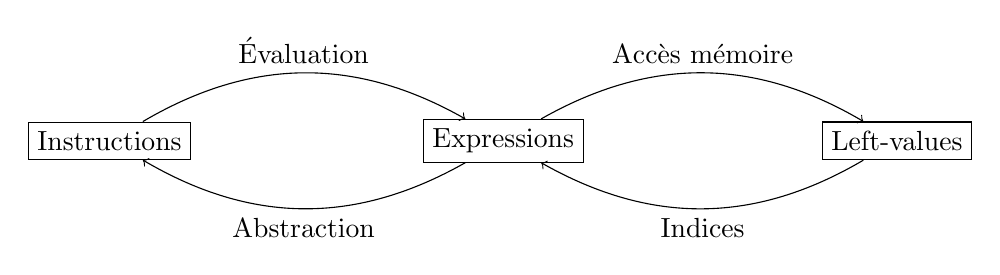
\begin{tikzpicture}
[node distance=5cm]

\node[draw] (I) {Instructions};

\node[draw, right of=I] (E) {Expressions};

\node[draw, right of=E] (L) {Left-values};

\draw[->] (I) edge[bend left] node[auto] {Évaluation} (E);
\draw[->] (E) edge[bend left] node[auto] {Abstraction} (I);
\draw[->] (E) edge[bend left] node[auto] {Accès mémoire} (L);
\draw[->] (L) edge[bend left] node[auto] {Indices} (E);

\end{tikzpicture}
\end{center}

\begin{theorem}[Progrès]
\label{thm:progres}

Supposons que $Γ ⊢ i$. Soit $m$ un état mémoire tel que $\mcomp{Γ}{m}$.

Alors l'un des cas suivants est vrai:
\begin{itemize}
\item $i = \iPass$
\item $∃v, i = \iReturn{v}$
\item $∃ (i', m'), \mm{m}{i}{m'}{i'}$
\item $∃ Ω ∈ \{\serr{div},\serr{array},\serr{ptr}\}, \msi{m}{i} → Ω$
\end{itemize}

\jolibreak

  Supposons que $Γ ⊢ e : t$. Soit $m$ un état mémoire tel que $\mcomp{Γ}{m}$.
  Alors l'un des cas suivant est vrai:

\begin{itemize}
  \item $∃ v ≠ Ω, e = v$
  \item $∃ (e', m'), \mm{m}{e}{m'}{e'}$
  \item $∃ Ω ∈ \{\serr{div},\serr{array},\serr{ptr}\}, \msi{m}{e} → Ω$
\end{itemize}

\jolibreak

Supposons que $Γ ⊢ lv : t$. Soit $m$ un état mémoire tel que $\mcomp{Γ}{m}$.

Alors l'un des cas suivants est vrai:
\begin{itemize}
\item $∃φ, lv = φ$
\item $∃ (lv', m'), \mm{m}{lv}{m'}{lv'}$
\item $∃ Ω ∈ \{\serr{div},\serr{array},\serr{ptr}\}, \msi{m}{lv} → Ω$
\end{itemize}

\end{theorem}

C'est-à-dire, soit:

\begin{itemize}
  \item l'entité (instruction, expression ou left-value) est complètement
évaluée.
  \item un pas d'évaluation est possible.
  \item une erreur de division, tableau ou pointeur se produit.
\end{itemize}

La preuve du théorème~\ref{thm:progres} se trouve en annexe~\ref{proof:progres}.

\begin{lemma}[Représentabilité]
\label{lemma:repr}

On définit un opérateur de représentation d'un type statique à l'exécution:

    \begin{align*}
        \cRepr{ \tInt   } &= \tInt   \\
        \cRepr{ \tFloat } &= \tFloat \\
        \cRepr{ \tUnit  } &= \tUnit  \\
        \cRepr{ t'*      } &= \cRepr{t'}* \\
        \cRepr{ t'[]     } &= \cRepr{t'}[] \\
        \cRepr{ \tStruct{ l_1 : t_1; … ; l_n : t_n } }
        &= \tStruct{ l_1 : \cRepr{t_1}; … ; l_n : \cRepr{t_n} }\\
        \cRepr{ (t_1, …, t_n) \rightarrow t } &= \stFun{n}
    \end{align*}

Supposons que $Γ ⊢ v : t$ et $\mcomp{Γ}{m}$.
On pose $τ = \cRepr{t}$.
Alors $m ⊧ v : τ$ et $\tComp{τ}{t}$.

\end{lemma}

\begin{proof}%{{{

On procède par induction sur la forme de $t$.

\begin{itemize}
\item $\tInt$:
    D'après le lemme des formes canoniques, $v = n$.
    On conclut avec \textsc{S-Int} et \textsc{Comp-Ground}.

\item $\tFloat$:
    Idem avec $v = d$ et \textsc{S-Float}.

\item $\tUnit$:
    Idem avec $v = \eUnit$ et \textsc{S-Unit}.

\item $t = t'*$:
    Soient $τ' = \cRepr{t'}$ et $τ = τ'~*$.
    D'après le lemme des formes canoniques, deux cas sont possibles:

    \begin{itemize}
        \item $v = \widehat{\&}~φ$:

            Par inversion, $Γ ⊢ φ : t'$

            Puisque $\mcomp{Γ}{m}$ et $Φ ⊢ φ : t'$, on obtient par le
            lemme~\ref{lemma:mem-typ} que
            $m[φ]_Φ$ est une valeur telle que
            $m ⊧ m[φ]_Φ : τ'$ où $\tComp{τ'}{t'}$.
            D'après \textsc{S-Ptr}, $m ⊧ \widehat{\&}~φ : τ$.

            De plus par \textsc{Comp-Ptr}
            $\tComp{τ}{t}$.

        \item $v = \eNull$:

            Par induction, $\tComp{τ'}{t'}$. Alors par \textsc{Comp-Ptr},
            $\tComp{τ~*}{t~*}$.

            En outre, grâce à \textsc{S-Null}, on obtient $m ⊧ \eNull: τ~*$.

    \end{itemize}

\item $t = t'[]$:
    Par le lemme des formes canoniques,
    $v = \widehat{\eArray{v_1,…,v_n}}$.
    Par inversion on obtient que $∀i, Γ ⊢ v_i : t'$.

    Soient $τ' = \cRepr{t'}$ et $τ = τ'~[]$.

    Alors par induction $∀i, m ⊧ v_i : τ'$ et $\tComp{τ}{t}$.
    De la première propriété il vient (via \textsc{S-Array})
    $m ⊧ v : τ$, et de la seconde (via \textsc{Comp-Array})
    $\tComp{τ}{t}$.

\item $\tStruct{ l_1 : t_1; … ; l_n : t_n }$:
    Par le lemme des formes canoniques,
    $v = \widehat{\eStruct{l_1:v_1;…;l_n:v_n}}$.
    Et par inversion, $∀i, Γ ⊢ v_i : t_i$.

    Soient $τ_i = \cRepr{t_i}$ et
    $τ = \tStruct{ l_1 : τ_1; … ; l_n : τ_n }$.

    Alors par induction, $∀i, m ⊧ v_i : τ_i$ et $\tComp{τ_i}{t_i}$.

    On déduit de \textsc{S-Struct} que $m ⊧ v : τ$, et de
    \textsc{Comp-Struct} que $\tComp{τ}{t}$.

\item $t = (t_1, …, t_n) \rightarrow t'$:
    Par formes canoniques, on a
    $v = \widehat{\eFun{a_1,…,a_n}{i}}$.

    Soit $τ = \stFun{n}$: par \textsc{S-Fun} on obtient que
    $m ⊧ v : τ$. On conclut d'autre part que $\tComp{τ}{t}$
    grâce à \textsc{Comp-Fun}.

\end{itemize}
\end{proof}%}}}

% attention il est recopié dans d-preuves

\begin{theorem}[Préservation]
\label{thm:preservation}

Soient $Γ$ un environnement de typage, et $m$ un état mémoire tels que
$\mcomp{Γ}{m}$.

Alors:

\begin{itemize}
\item
    Si $Γ ⊢ lv : t$ et $\mm{m}{lv}{m'}{φ}$,
    alors $\mcomp{Γ}{\cCleanup{m'}}$ et $\semtypphi{m'}{φ}{τ}$ où $\tComp{τ}{t}$.

\item
    Si $Γ ⊢ lv : t$ et $\mm{m}{lv}{m'}{lv'}$,
    alors $\mcomp{Γ}{\cCleanup{m'}}$ et $Γ ⊢ lv' : t$.

\item
    Si $Γ ⊢ e : t$ et $\mm{m}{e}{m'}{v}$,
    alors $\mcomp{Γ}{\cCleanup{m'}}$ et $m' ⊧ v : τ$ où $\tComp{τ}{t}$.

\item
    Si $Γ ⊢ e : t$ et $\mm{m}{e}{m'}{e'}$,
    alors $\mcomp{Γ}{\cCleanup{m'}}$ et $Γ ⊢ e' : t$.

\item
    Si $Γ ⊢ i$ et $\mm{m}{i}{m'}{i'}$,
    alors $\mcomp{Γ}{\cCleanup{m'}}$ et $Γ ⊢ i'$.
\end{itemize}

  Autrement dit, si une construction est typable, alors un pas d'évaluation ne
  modifie pas son type et préserve le typage de la mémoire.

\end{theorem}

\paragraph{Remarque}

Dans la formulation classique de ce théorème, on indique que $\mcomp{Γ}{m}$
implique $\mcomp{Γ}{m'}$. Ici, la conclusion est moins forte en indiquant
seulement que $\mcomp{Γ}{\cCleanup{m'}}$. Cela indique que la compatibilité
mémoire est établie mais peut localement introduire des pointeurs fous. En fait,
comme une étape de $\phx\cCleanup$ est faite après chaque appel de fonction et
chaque déclaration, la propriété classique est vraie mais uniquement sur un plus
grand pas d'exécution.

La preuve de ce théorème se trouve en annexe~\ref{proof:preservation}.

Cela prouve qu'aucun terme ne reste «bloqué» parce qu'aucune règle ne
s'applique, et que la sémantique respecte le typage. En quelque sorte, les types
sont un contrat entre les expressions et les fonctions: si leur évaluation
converge, alors une valeur du type inféré sera produite.

Enfin, on donne une version de ces propriétés pour les phrases de programme.

\begin{theorem}[Progrès pour les phrases]
\label{thm:prog-phr}

Soient $Γ$ un environnement de typage, $m$ un état mémoire et $p$ une phrase de
programme. Supposons que $\typh{Γ}{p}{Γ'}$ et $\mcomp{Γ}{m}$.

On suppose en outre que l'évaluation de $p$ termine.

Alors $∃ m'. \ph{m}{p}{m'}$.

\end{theorem}

\begin{proof}

Ici il n'y a pas de difficulté puisque la contrainte (forte) de terminaison se
lit $\mm{m}{e}{m'}{v'}$ où $e$ est l'expression apparaissant dans $p$.

Selon la forme de $p$, il suffit alors d'appliquer la règle
\textsc{ET-Exp} ou \textsc{ET-Var}.

\end{proof}

\begin{theorem}[Préservation pour les phrases]
\label{thm:presa-phr}

On suppose que les trois propriétés suivantes sont vérifiées:

\[
\begin{cases}
    \mcomp{Γ}{m} \\
    \typh{Γ}{p}{Γ'} \\
    \ph{m}{p}{m'}
\end{cases}
\]

Alors $\mcomp{Γ'}{m'}$.

\end{theorem}

\begin{proof}

On distingue selon la dernière règle appliquée dans la dérivation de
$\ph{m}{p}{m'}$.

\paragraph{\textsc{ET-Exp}:}%{{{
La dernière règle appliquée pour dériver $\typh{Γ}{p}{Γ'}$ est donc
\textsc{T-Exp}. D'après les prémisses de ces deux règles, on a donc
$Γ ⊢ e : t$ et $\mm{m}{e}{m'}{v}$. Alors, d'après le théorème de préservation,
$\mcomp{Γ}{m'}$.
%}}}
\paragraph{\textsc{ET-Var}:}%{{{

Ici, la dérivation de $\typh{Γ}{p}{Γ'}$ termine par \textsc{T-Var}.
D'après leurs prémisses, on a donc :
$Γ ⊢ e : t$, $Γ' = \extendGlobal{Γ}{x}{t}$, et
$m'' = (s, (x ↦ v)::g)$ où $(s, g) = m'$
(on cherche à prouver que $\mcomp{Γ'}{m''}$).

En appliquant le théorème de préservation, on obtient que $Γ ⊢ v : t$ et
$\mcomp{Γ}{m'}$. D'après le lemme~\ref{lemma:repr}, il existe $τ$ tel que
$m' ⊧ v : τ$ où $\tComp{τ}{t}$. On peut alors appliquer \textsc{M-Global} qui
nous donne que $\mcomp{Γ'}{m''}$.
% }}}

\end{proof}

\section*{Conclusion}

On ajoute un système de types statiques à \langname. Cela permet de calculer à
la compilation la forme des valeurs produite par chaque expression. Pour ce
faire on définit un ensemble de règles de typage (regroupées dans
l'annexe~\ref{anx:typage}) à appliquer selon la forme de celle-ci.

Si on considère des programmes qui sont seulement syntaxiquement corrects, on ne
ne peut rien prédire sur leur exécution. Par exemple, $\eFun{x}{\iPass} + 1$ est
une expression correcte mais pour laquelle il n'y a pas de règle d'évaluation
qui s'applique. En ajoutant un système de type, les propriétés de sûreté
établies dans ce chapitre assurent que les termes peuvent être évalués, et que
les valeurs produites sont en accord avec les types données aux différentes
parties du programme. Cela permet surtout de s'assurer que les programmes ne
peuvent provoquer une erreur d'exécution que dans certains cas particuliers,
comme les division ou les accès aux tableaux.

À l'issue de ce chapitre, on a donc un langage impératif sain pour bâtir de
nouvelles analyses de typage, ce que nous allons faire dans le chapitre
suivant.

% vim: spelllang=fr
